\chapter{GAMBARAN UMUM PERUSAHAAN}
% DOCX block 286
\section{Sejarah Singkat Perusahaan}

% DOCX block 287
\subsection{Profil Perusahaan}

% DOCX block 288
PT XYZ berlokasi di Kabupaten Mojokerto, Provinsi Jawa Timur. Perusahaan berada di kawasan industri yang terhubung dengan jalur logistik di Jawa Timur sehingga mendukung distribusi produk dan penerimaan bahan baku.

% DOCX block 289
Kegiatan utama PT XYZ adalah manufaktur komponen otomotif, khususnya wiring harness atau rangkaian kabel kelistrikan kendaraan. Produk ini menghubungkan berbagai komponen elektronik serta menyalurkan daya dan sinyal agar fungsi kelistrikan kendaraan dapat bekerja sesuai rancangan.

% DOCX block 290
PT XYZ berafiliasi dengan korporasi induk yang berpusat di Jepang dan menjadi bagian dari jaringan pemasok komponen untuk industri otomotif. Kegiatan manufakturnya menuntut ketelitian perakitan, kesesuaian spesifikasi pelanggan, serta pengendalian mutu pada setiap tahapan produksi.

% DOCX block 291
\subsection{Sejarah Perusahaan}

% DOCX block 292
Perkembangan industri otomotif meningkatkan kebutuhan terhadap sistem kelistrikan kendaraan yang semakin kompleks. Korporasi induk PT XYZ di Jepang mengembangkan jaringan produksi wiring harness untuk memenuhi kebutuhan pasar di berbagai negara. Sebagai bagian dari pengembangan jaringan tersebut, PT XYZ didirikan di Mojokerto, Jawa Timur, pada tahun 2002 untuk mendukung permintaan pasar domestik dan ekspor.

% DOCX block 293
Perusahaan memperbaiki metode kerja dan menggunakan teknologi dalam proses manufaktur. Perakitan produk memerlukan peralatan yang siap digunakan, pengawasan proses, dan pemeriksaan mutu agar hasilnya memenuhi persyaratan pelanggan.

% DOCX block 294
Pemeliharaan mesin diperlukan agar peralatan produksi tetap siap digunakan. Data kondisi mesin membantu personel Maintenance meninjau perubahan yang terjadi selama mesin beroperasi.

Perusahaan menargetkan produksi tanpa cacat (\textit{zero defect}). Divisi
Maintenance mendukung sasaran ini dengan menjaga kesiapan mesin dan
menelusuri perubahan parameter saat mesin beroperasi.

% DOCX block 295
\subsection{Filosofi Perusahaan}

% DOCX block 296
Filosofi perusahaan mengacu pada kebijakan korporasi induk di Jepang yang terdiri atas dua prinsip, yaitu ``A Corporation in Step with the World'' dan ``A Corporation Needed by Society''. Kedua prinsip tersebut menjadi landasan budaya kerja dan arah pengembangan perusahaan.

% DOCX block 297
Prinsip ``A Corporation in Step with the World'', yang berarti perusahaan yang melangkah bersama dunia, menekankan kemampuan mengikuti perkembangan teknologi, memahami kebutuhan pelanggan, dan menyesuaikan diri terhadap perubahan lingkungan usaha. Dalam kegiatan manufaktur, prinsip ini diwujudkan melalui penyempurnaan proses produksi dan pengembangan cara kerja yang mendukung mutu serta efisiensi.

% DOCX block 298
Prinsip ``A Corporation Needed by Society'', yang berarti perusahaan yang dibutuhkan oleh masyarakat, menempatkan manfaat kegiatan usaha bagi masyarakat sebagai bagian dari tanggung jawab perusahaan. Pembukaan kesempatan kerja, pengembangan keterampilan sumber daya manusia, serta keterlibatan dalam kegiatan ekonomi merupakan bentuk kontribusi yang diuraikan dalam profil perusahaan.

% DOCX block 299
Kedua prinsip tersebut mengarahkan perusahaan untuk menjaga mutu produk, mengikuti perkembangan industri, dan memperhatikan tanggung jawab sosial.

% DOCX block 300
\section{Struktur Organisasi}

% DOCX block 301
Struktur organisasi PT XYZ membagi tugas ke dalam fungsi produksi, persiapan produksi, rekayasa, mutu, logistik, keuangan, sumber daya manusia, dan urusan umum. Setiap unit mempunyai tanggung jawab masing-masing dan berkoordinasi dengan unit lain.

% DOCX block 302
Fungsi Maintenance termasuk dalam bidang Mechanical Engineer atau Engineering, bersama fungsi rekayasa produksi dan pengelolaan peralatan. Maintenance bertanggung jawab terhadap pemeliharaan dan perbaikan mesin. Kedudukan ini berkaitan langsung dengan kegiatan penulis dalam pengembangan monitoring parameter mesin cutting.

% DOCX block 303
Pelaksanaan kerja praktik dibimbing oleh Imsyar Lubis Tandika selaku pembimbing lapangan, dengan Dwi Jasmianto sebagai Senior Manager. Arahan pekerjaan dan evaluasi hasil dilakukan melalui pembimbing lapangan. Bagan struktur organisasi ditempatkan pada Gambar~\ref{fig:draft-2-1}.

% DOCX block 304
\begin{figure}[H]
  \centering
  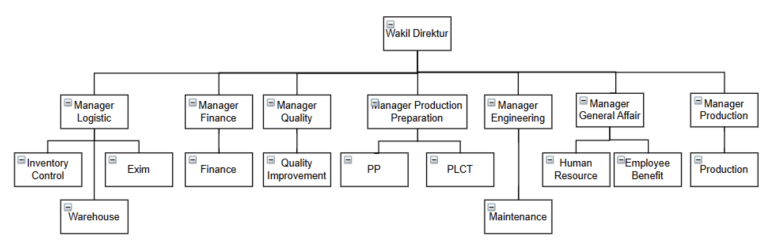
\includegraphics[width=\linewidth]{assets/gambar/gambar-2-01.png}
  \caption{Struktur organisasi PT XYZ}\label{fig:draft-2-1}
  \end{figure}

% DOCX block 305
\section{Hak dan Wewenang}

% DOCX block 306
Pembagian tugas dan wewenang perusahaan mengikuti struktur fungsional. Uraian setiap jabatan dan divisi disajikan sebagai berikut.

% DOCX block 307
\subsection{President Director atau Presiden Direktur}

% DOCX block 308
Presiden Direktur memimpin perusahaan dan menetapkan kebijakan usaha. Tugasnya meliputi pengawasan kegiatan operasional, pengendalian internal, serta penetapan rencana usaha sesuai perkembangan pasar.

% DOCX block 309
\subsection{Vice President Director atau Wakil Presiden Direktur}

% DOCX block 310
Wakil Presiden Direktur membantu Presiden Direktur memimpin perusahaan. Ia mengoordinasikan unit kerja agar kegiatan sehari-hari mengikuti kebijakan dan sasaran perusahaan.

% DOCX block 311
\subsection{Division Personnel and General Affairs atau PGA}

% DOCX block 312
Divisi PGA mengelola sumber daya manusia dan fasilitas pendukung operasional perusahaan. Lingkup kegiatannya meliputi seksi-seksi berikut.

% DOCX block 313
\begin{enumerate}[leftmargin=*,itemsep=2pt]
\item Human Resource and Industrial Relationship: Menangani rekrutmen, administrasi kepegawaian, hubungan industrial, serta pengembangan kompetensi karyawan.

% DOCX block 314
\item General Affairs: Mengelola kebutuhan umum perusahaan, aset, keamanan, dan hubungan dengan instansi pemerintah maupun pihak eksternal.

% DOCX block 315
\item Interpreter: Mendukung penerjemahan bahasa untuk memperlancar komunikasi internal dan eksternal.

% DOCX block 316
\item Employee Benefit: Mengelola kompensasi, fasilitas, dan tunjangan kesejahteraan karyawan.

% DOCX block 317
\item Safety Health and Environment: Mendukung penerapan keselamatan dan kesehatan kerja serta pengelolaan lingkungan di area perusahaan.

% DOCX block 318
\end{enumerate}

\subsection{Division Finance Accounting atau FA}

% DOCX block 319
Divisi Finance Accounting mengelola pencatatan dan arus keuangan perusahaan, termasuk penerimaan, pengeluaran, dan pelaporannya. Divisi ini meliputi seksi berikut.

% DOCX block 320
\begin{enumerate}[leftmargin=*,itemsep=2pt]
\item Finance and Accounting: Melakukan pencatatan transaksi, menyusun laporan keuangan berkala, serta menangani administrasi kewajiban perpajakan.

% DOCX block 321
\item Custom Document Control: Mengelola dokumen dan perizinan yang berkaitan dengan kegiatan kepabeanan.

% DOCX block 322
\end{enumerate}

\subsection{Division Quality Assurance atau QA}

% DOCX block 323
Divisi Quality Assurance memastikan kesesuaian produk dengan persyaratan mutu yang ditetapkan perusahaan dan pelanggan. Lingkup pengawasannya meliputi seksi berikut.

% DOCX block 324
\begin{enumerate}[leftmargin=*,itemsep=2pt]
\item Quality Assurance and Quality Control: Melakukan pemeriksaan bahan masuk, pengawasan proses produksi, serta pemeriksaan produk sebelum dikirim.

% DOCX block 325
\item Quality Improvement and Quality System Administration: Mengembangkan perbaikan sistem mutu serta memelihara administrasi dan dokumentasi sistem kualitas.

% DOCX block 326
\end{enumerate}

\subsection{Department Production atau PRO}

% DOCX block 327
Departemen Produksi menjalankan dan mengawasi proses manufaktur di lantai produksi, mulai dari persiapan bahan sampai produk siap diteruskan ke tahap berikutnya. Tugasnya mencakup pencapaian target keluaran harian, pemeliharaan kesesuaian proses, dan koordinasi kegiatan agar aliran produksi tetap lancar.

% DOCX block 328
\subsection{Division Production Preparation atau PP}

% DOCX block 329
Divisi Production Preparation mempersiapkan kebutuhan sebelum proses produksi massal dilaksanakan. Kegiatan tersebut didukung oleh seksi berikut.

% DOCX block 330
\begin{enumerate}[leftmargin=*,itemsep=2pt]
\item Production Preparation: Menyusun dokumen perencanaan produksi, menyiapkan tata letak area kerja, alat bantu, serta instruksi kerja.

% DOCX block 331
\item Program Launch Coordinator: Mengoordinasikan persiapan peluncuran model produk baru dengan unit-unit terkait.

% DOCX block 332
\item Design Engineering: Menerjemahkan spesifikasi teknis pelanggan menjadi data dan kebutuhan produksi yang dapat diterapkan.

% DOCX block 333
\end{enumerate}

\subsection{Division NYS dan Training}

% DOCX block 334
Divisi NYS dan Training mendukung pengembangan sistem kerja internal serta keterampilan karyawan. Divisi ini mencakup seksi berikut.

% DOCX block 335
\begin{enumerate}[leftmargin=*,itemsep=2pt]
\item NYS: Mengembangkan dan menerapkan sistem manajemen produksi sesuai kebijakan korporasi.

% DOCX block 336
\item Training: Menyelenggarakan pelatihan keterampilan teknis dan nonteknis bagi karyawan.

% DOCX block 337
\item Local Purchase: Menangani pengadaan barang dan jasa dari pemasok lokal untuk memenuhi kebutuhan perusahaan.

% DOCX block 338
\item Information Technology: Memelihara infrastruktur teknologi informasi, perangkat keras, perangkat lunak, dan jaringan perusahaan.

% DOCX block 339
\end{enumerate}

\subsection{Division Mechanical Engineer atau ME}

% DOCX block 340
Divisi Mechanical Engineer mendukung kesiapan teknis fasilitas produksi. Lingkup pekerjaannya mencakup seksi berikut.

% DOCX block 341
\begin{enumerate}[leftmargin=*,itemsep=2pt]
\item Maintenance: Melaksanakan pemeliharaan preventif dan perbaikan mesin industri serta peralatan pabrik.

% DOCX block 342
\item Production Engineering: Menangani rekayasa lini produksi, penerapan otomasi, serta perbaikan teknis untuk mendukung kelancaran proses.

% DOCX block 343
\item Stock and Equipment Control: Mengelola persediaan suku cadang mesin dan peralatan teknik.

% DOCX block 344
\end{enumerate}

\subsection{Division Logistic}

% DOCX block 345
Divisi Logistik mengelola kegiatan rantai pasok dan distribusi. Tanggung jawabnya terbagi dalam seksi berikut.

% DOCX block 346
\begin{enumerate}[leftmargin=*,itemsep=2pt]
\item Production Planning and Control: Menyusun jadwal produksi serta mengoordinasikan kebutuhan bahan baku sesuai rencana produksi.

% DOCX block 347
\item Export and Import: Menangani pengiriman produk ekspor dan penerimaan bahan baku impor.

% DOCX block 348
\item Inventory Control and Warehouse: Mengelola penyimpanan bahan baku dan produk jadi serta mengendalikan perputaran persediaan.

% DOCX block 349
\end{enumerate}

Pelaksanaan kerja praktik penulis berada pada Divisi Maintenance. Arahan teknis dan evaluasi pekerjaan diberikan oleh Imsyar Lubis Tandika selaku pembimbing lapangan, dengan Dwi Jasmianto sebagai Senior Manager.

% DOCX block 350
\Needspace{13.5cm}
\section{Lokasi Perusahaan}

% DOCX block 351
PT XYZ berlokasi di Kecamatan Ngoro, Kabupaten Mojokerto, Provinsi Jawa Timur. Perusahaan berada di kawasan industri yang berdekatan dengan wilayah Kabupaten Pasuruan dan Sidoarjo. Kedudukan tersebut mendukung hubungan perusahaan dengan jaringan logistik di Jawa Timur.

% DOCX block 352
Peta lokasi perusahaan ditunjukkan pada Gambar~\ref{fig:draft-2-2}.

% DOCX block 353
\GambarLaporan{assets/gambar/gambar-2-02.png}{Lokasi PT XYZ}{fig:draft-2-2}{}

% DOCX block 354
\section{Kesehatan dan Keselamatan Kerja (K3)}

% DOCX block 355
\subsection{Pengertian}

% DOCX block 356
Keselamatan dan kesehatan kerja (K3) merupakan upaya pencegahan kecelakaan serta gangguan kesehatan yang berkaitan dengan pekerjaan. Dalam lingkungan manufaktur, penerapannya mencakup pengenalan bahaya, pengendalian risiko, penggunaan peralatan yang sesuai, dan pembentukan perilaku kerja yang aman. K3 menjadi bagian dari kegiatan operasional PT XYZ.

% DOCX block 357
Pada pekerjaan monitoring mesin cutting, perhatian keselamatan berkaitan dengan keberadaan panel listrik, bagian mekanis bergerak, permukaan panas, serta sistem udara bertekanan. Pengembangan sistem monitoring tetap mengikuti kewenangan kerja dan ketentuan keselamatan perusahaan.

% DOCX block 358
\subsection{Tujuan}

% DOCX block 359
Penerapan K3 bertujuan melindungi pekerja, mencegah kerusakan peralatan, dan mendukung keberlangsungan kegiatan produksi. Lingkungan kerja yang tertib membantu mengurangi kemungkinan paparan bahaya serta memudahkan pelaksanaan pekerjaan secara terencana.

% DOCX block 360
Dalam kegiatan kerja praktik, tujuan tersebut berkaitan dengan keselamatan saat observasi, pemasangan perangkat, pemeriksaan koneksi, dan pengujian. Pekerjaan teknis dikoordinasikan dengan pembimbing atau personel yang berwenang sesuai jenis tugas dan sumber energi yang terlibat.

% DOCX block 361
\subsection{Komitmen Keselamatan}

% DOCX block 362
Komitmen keselamatan perusahaan menjadi pedoman dalam melaksanakan pekerjaan sehari-hari. Pokok komitmen yang dijelaskan dalam kebijakan keselamatan perusahaan meliputi hal-hal berikut.

% DOCX block 363
\begin{enumerate}[leftmargin=*,itemsep=2pt]
\item Memastikan area kerja berada dalam kondisi aman sebelum dan sesudah pekerjaan dengan menerapkan prinsip 5S atau 5R.

% DOCX block 364
\item Menggunakan alat pelindung diri secara tepat sesuai jenis pekerjaan dan ketentuan area kerja.

% DOCX block 365
\item Melaksanakan pekerjaan berdasarkan petunjuk kerja dengan penuh tanggung jawab.

% DOCX block 366
\item Segera melaporkan dan mengingatkan apabila ditemukan kondisi atau perilaku yang tidak aman.

% DOCX block 367
\item Meningkatkan kewaspadaan terhadap potensi bahaya dan penyakit akibat kerja.

% DOCX block 368
\end{enumerate}

\subsection{Istilah Bahaya di Lingkungan Kerja}

% DOCX block 369
Pemahaman istilah bahaya diperlukan agar pekerja dapat mengenali sumber masalah dan menyampaikan kondisi keselamatan dengan jelas. Istilah yang berkaitan dengan keselamatan kerja meliputi hal-hal berikut.

% DOCX block 370
\subsubsection{Hazard}

% DOCX block 371
Hazard merupakan sumber atau keadaan yang berpotensi menyebabkan cedera, gangguan kesehatan, kerusakan, atau gangguan terhadap pelaksanaan pekerjaan.

% DOCX block 372
\subsubsection{Danger}

% DOCX block 373
Danger menggambarkan keadaan berbahaya yang memerlukan perhatian dan pengendalian agar tidak berkembang menjadi kejadian yang merugikan.

% DOCX block 374
\subsubsection{Risk}

% DOCX block 375
Risk atau risiko berkaitan dengan kemungkinan terjadinya kejadian dan tingkat keparahan akibat yang dapat ditimbulkannya.

% DOCX block 376
\subsubsection{Incident}

% DOCX block 377
Incident merupakan kejadian yang berkaitan dengan pekerjaan dan dapat menimbulkan kerugian atau memiliki potensi menimbulkan kerugian.

% DOCX block 378
\subsubsection{Accident}

% DOCX block 379
Accident merupakan kejadian yang menimbulkan cedera, gangguan kesehatan, kerusakan, atau kerugian lainnya.

% DOCX block 380
Dalam kegiatan manufaktur wiring harness, pengendalian bahaya mencakup kondisi mesin, peralatan listrik, bahan yang digunakan, serta perilaku kerja. Pengenalan bahaya menjadi dasar penentuan tindakan pencegahan dan pelaporan kepada pihak yang berwenang.

% DOCX block 381
% Layout: gambar perlengkapan dibuat ringkas dan judul dijaga bersama uraiannya.
\setlength{\TinggiRuangGambar}{2.2cm}
\setlength{\BatasTinggiGambar}{3.2cm}
\subsection{Alat Pelindung Diri (APD)}

% DOCX block 382
Alat Pelindung Diri (APD) merupakan perlengkapan untuk melindungi seluruh atau sebagian tubuh dari paparan bahaya selama bekerja. Jenis APD yang dicantumkan dalam dokumentasi perusahaan diuraikan sebagai berikut. Penggunaan setiap perlengkapan mengikuti penilaian bahaya, spesifikasi produk, dan ketentuan perusahaan.

% DOCX block 383
\Needspace{6.8cm}
\subsubsection{Masker Shigematsu Seri GM76D}

% DOCX block 384
Masker Shigematsu Seri GM76D merupakan pelindung pernapasan yang tercantum dalam dokumentasi perusahaan. Jenis penyaring dipilih berdasarkan bahan atau partikel yang mungkin terhirup dan ketentuan keselamatan area kerja.

% DOCX block 385
\GambarLaporan{assets/gambar/gambar-2-03.png}{Masker Shigematsu Seri GM76D}{fig:draft-2-3}{}

% DOCX block 386
\Needspace{6.8cm}
\subsubsection{Masker 3M}

% DOCX block 387
Masker 3M digunakan sebagai pelindung pernapasan sesuai jenis dan spesifikasi produknya. Kesesuaian masker dengan paparan debu, partikel, atau bahan lain ditentukan berdasarkan penilaian bahaya di tempat kerja.

% DOCX block 388
\GambarLaporan{assets/gambar/gambar-2-04.png}{Masker 3M}{fig:draft-2-4}{}

% DOCX block 389
\Needspace{6.8cm}
\subsubsection{Kacamata Safety 3M Tipe 2750}

% DOCX block 390
Kacamata keselamatan melindungi mata saat bekerja. Jenis lensa dan tingkat perlindungannya dipilih berdasarkan bahaya pekerjaan dan petunjuk penggunaan produk.

% DOCX block 391
\GambarLaporan{assets/gambar/gambar-2-05.png}{Kacamata Safety 3M Tipe 2750}{fig:draft-2-5}{}

% DOCX block 392
\Needspace{6.8cm}
\subsubsection{Kacamata Safety Porsch}

% DOCX block 393
Kacamata keselamatan ini dicantumkan untuk pekerjaan yang berpotensi menghasilkan debu atau partikel, seperti pekerjaan pemesinan. Penggunaannya mengikuti ketentuan perlindungan mata pada area kerja terkait.

% DOCX block 394
\GambarLaporan{assets/gambar/gambar-2-06.png}{Kacamata Safety Porsch}{fig:draft-2-6}{}

% DOCX block 395
\Needspace{6.8cm}
\subsubsection{Kacamata Safety Yamamoto}

% DOCX block 396
Pelindung mata digunakan ketika pekerjaan berpotensi menimbulkan percikan bahan. Pemilihan bentuk dan spesifikasi pelindung disesuaikan dengan bahan yang digunakan serta ketentuan keselamatan proses.

% DOCX block 397
\GambarLaporan{assets/gambar/gambar-2-07.png}{Kacamata Safety Yamamoto}{fig:draft-2-7}{}

% DOCX block 398
\Needspace{6.8cm}
\subsubsection{Earmuff}

% DOCX block 399
Earmuff merupakan pelindung pendengaran yang menutup bagian luar telinga. Penggunaannya ditentukan berdasarkan penilaian kebisingan dan kebutuhan perlindungan pada area kerja.

% DOCX block 400
\GambarLaporan{assets/gambar/gambar-2-08.png}{Earmuff}{fig:draft-2-8}{}

% DOCX block 401
\Needspace{6.8cm}
\subsubsection{Earplug}

% DOCX block 402
Earplug merupakan pelindung pendengaran yang digunakan pada saluran telinga. Pemasangan yang benar dan kesesuaian jenis produk diperlukan agar perlindungan sesuai kebutuhan paparan kebisingan.

% DOCX block 403
\GambarLaporan{assets/gambar/gambar-2-09.png}{Earplug}{fig:draft-2-9}{}

% DOCX block 404
\Needspace{6.8cm}
\subsubsection{Face Shield Transparan}

% DOCX block 405
Face shield melindungi bagian wajah dari potensi percikan atau partikel yang timbul selama pekerjaan. Pemilihan bahan dan spesifikasinya mengikuti jenis paparan serta ketentuan penggunaan pelindung tambahan.

% DOCX block 406
\GambarLaporan{assets/gambar/gambar-2-10.png}{Face Shield Transparan}{fig:draft-2-10}{}

% DOCX block 407
\Needspace{6.8cm}
\subsubsection{Sarung Tangan Benang DUSAFE Tipe CWG 004}

% DOCX block 408
Sarung tangan digunakan untuk melindungi tangan selama penanganan material sesuai karakteristik pekerjaannya. Pemilihannya memperhatikan risiko permukaan material dan kemungkinan tersangkut pada bagian mesin yang bergerak.

% DOCX block 409
\GambarLaporan{assets/gambar/gambar-2-11.png}{Sarung Tangan Benang DUSAFE Tipe CWG 004}{fig:draft-2-11}{}

% DOCX block 410
\Needspace{6.8cm}
\subsubsection{Sarung Tangan Kulit DUSAFE Tipe CBB008}

% DOCX block 411
Sarung tangan kulit digunakan untuk melindungi tangan saat bekerja. Pemilihannya harus mengikuti risiko pekerjaan, kemampuan bahan sarung tangan, dan instruksi keselamatan yang berlaku.

% DOCX block 412
\GambarLaporan{assets/gambar/gambar-2-12.png}{Sarung Tangan Kulit DUSAFE Tipe CBB008}{fig:draft-2-12}{}

% DOCX block 413
\Needspace{6.8cm}
\subsubsection{Sarung Tangan Pelindung Bahan Kimia}

% DOCX block 414
Sarung tangan pelindung bahan kimia digunakan untuk mengurangi kontak langsung antara kulit dan bahan yang ditangani. Bahan sarung tangan dipilih berdasarkan kesesuaiannya dengan bahan kimia atau pelumas yang digunakan.

% DOCX block 415
\GambarLaporan{assets/gambar/gambar-2-13.png}{Sarung Tangan Pelindung Bahan Kimia}{fig:draft-2-13}{}

% DOCX block 416
\Needspace{6.8cm}
\subsubsection{Helm Safety}

% DOCX block 417
Helm keselamatan melindungi kepala dari potensi benturan atau benda jatuh sesuai kelas perlindungannya. Kondisi cangkang dan sistem penyangga helm perlu diperiksa sebelum digunakan.

% DOCX block 418
\GambarLaporan{assets/gambar/gambar-2-14.png}{Helm Safety}{fig:draft-2-14}{}

% DOCX block 419
\Needspace{6.8cm}
\subsubsection{Welding Shield}

% DOCX block 420
Welding shield merupakan pelindung wajah dan mata untuk pekerjaan pengelasan. Tingkat perlindungan lensa dan kelengkapan APD pengelasan disesuaikan dengan jenis proses yang dilakukan.

% DOCX block 421
\GambarLaporan{assets/gambar/gambar-2-15.png}{Welding Shield}{fig:draft-2-15}{}

% DOCX block 422
\Needspace{6.8cm}
\subsubsection{Sepatu Safety}

% DOCX block 423
Sepatu keselamatan melindungi kaki dari risiko pekerjaan sesuai spesifikasinya. Pemilihan sepatu mempertimbangkan bahaya benturan, benda tajam, kondisi permukaan lantai, dan kebutuhan area kerja.

% DOCX block 424
\GambarLaporan{assets/gambar/gambar-2-16.png}{Sepatu Safety}{fig:draft-2-16}{}

% DOCX block 425
\Needspace{6.8cm}
\subsubsection{Boot Safety}

% DOCX block 426
Boot keselamatan digunakan pada pekerjaan yang memerlukan perlindungan kaki dengan bentuk dan bahan yang sesuai. Ketahanan bahan terhadap cairan serta kondisi permukaan kerja menjadi pertimbangan pemilihannya.

% DOCX block 427
\GambarLaporan{assets/gambar/gambar-2-17.png}{Boot Safety}{fig:draft-2-17}{}

% DOCX block 428
\Needspace{6.8cm}
\subsubsection{Apron}

% DOCX block 429
Apron melindungi bagian depan tubuh dan pakaian dari paparan selama pekerjaan. Jenis bahan apron disesuaikan dengan proses kerja, antara lain penanganan bahan, percikan, atau kebutuhan kebersihan.

% DOCX block 430
\GambarLaporan{assets/gambar/gambar-2-18.png}{Apron}{fig:draft-2-18}{}

% DOCX block 431
\Needspace{6.8cm}
\subsubsection{Body Harness}

% DOCX block 432
Body harness merupakan bagian dari perlengkapan perlindungan untuk pekerjaan pada ketinggian. Penggunaannya mengikuti sistem perlindungan jatuh, pemeriksaan perlengkapan, dan prosedur kerja yang ditetapkan perusahaan.

% DOCX block 433
\GambarLaporan{assets/gambar/gambar-2-19.png}{Body Harness}{fig:draft-2-19}{}

% DOCX block 434
\subsection{Bidang Kebakaran}

% DOCX block 435
Kebakaran merupakan kejadian api yang tidak dikehendaki dan memerlukan penanganan. Pencegahan dilakukan dengan mengendalikan sumber panas, bahan yang mudah terbakar, serta kondisi lingkungan kerja. PT XYZ menyediakan sarana keselamatan untuk mendukung tanggap darurat di area pabrik dan kantor.

% DOCX block 436
\Needspace{6.8cm}
\subsubsection{Alat Pemadam Api Ringan}

% DOCX block 437
Alat Pemadam Api Ringan (APAR) merupakan sarana pemadaman awal. Jenis media dan penggunaannya mengikuti karakteristik bahaya, petunjuk alat, serta pelatihan yang diberikan perusahaan.

% DOCX block 438
\GambarLaporan{assets/gambar/gambar-2-20.png}{Alat Pemadam Api Ringan}{fig:draft-2-20}{}

% DOCX block 439
\Needspace{6.8cm}
\subsubsection{Hydrant}

% DOCX block 440
Hydrant merupakan instalasi penyediaan air untuk mendukung penanganan kebakaran. Pengoperasiannya dilakukan oleh petugas yang berwenang sesuai prosedur tanggap darurat.

% DOCX block 441
\GambarLaporan{assets/gambar/gambar-2-21.png}{Hydrant}{fig:draft-2-21}{}

% DOCX block 442
\Needspace{6.8cm}
\subsubsection{Sensor Deteksi Asap dan Sistem Pemadam Ruangan}

% DOCX block 443
Detektor asap memberi peringatan awal ketika terdeteksi tanda kebakaran. Sistem deteksi dan pemadam ruangan digunakan sebagai bagian dari penanganan keadaan darurat.

% DOCX block 444
\GambarLaporan{assets/gambar/gambar-2-22.png}{Sensor Deteksi Asap dan Sistem Pemadam Ruangan}{fig:draft-2-22}{}

% DOCX block 445
\Needspace{6.8cm}
\subsubsection{Tanda Jalur Evakuasi}

% DOCX block 446
Tanda jalur evakuasi menunjukkan arah keluar menuju lokasi aman dalam keadaan darurat. Akses pada jalur tersebut perlu dijaga agar dapat digunakan sesuai rencana evakuasi perusahaan.

% DOCX block 447
\GambarLaporan{assets/gambar/gambar-2-23.png}{Tanda Jalur Evakuasi}{fig:draft-2-23}{}

% DOCX block 448
\Needspace{6.8cm}
\subsubsection{Titik Kumpul}

% DOCX block 449
Titik kumpul merupakan lokasi berkumpul setelah evakuasi. Lokasi ini digunakan untuk pendataan penghuni dan koordinasi petugas dalam memastikan kondisi personel.

% DOCX block 450
\GambarLaporan{assets/gambar/gambar-2-24.png}{Titik Kumpul}{fig:draft-2-24}{}

% DOCX block 451
\Needspace{6.8cm}
\subsubsection{Alarm Bahaya}

% DOCX block 452
Alarm bahaya memberikan peringatan mengenai keadaan darurat. Pekerja perlu mengenali tanda peringatan dan mengikuti instruksi petugas sesuai prosedur perusahaan.

% DOCX block 453
\GambarLaporan{assets/gambar/gambar-2-25.png}{Alarm Bahaya}{fig:draft-2-25}{}

% DOCX block 454
\setlength{\TinggiRuangGambar}{3.2cm}
\setlength{\BatasTinggiGambar}{0.58\textheight}
\begingroup
% Layout: bagian etika dimulai dengan ruang cukup, tanpa paragraf tersisa sendiri.
\titlespacing*{\section}{0pt}{8pt}{2pt}
\titlespacing*{\subsection}{0pt}{4pt}{2pt}
\Needspace{5cm}
\section{Etika Profesi}

% DOCX block 455
Etika profesi di PT XYZ mendukung budaya kerja dan pelaksanaan kegiatan operasional melalui prinsip berikut.

% DOCX block 456
\subsection{Integritas dan Kejujuran}

% DOCX block 457
Pekerjaan dan pelaporan dilaksanakan secara jujur. Kondisi pembacaan, hasil pengujian, dan keterbatasan sistem monitoring disampaikan sesuai fakta serta dapat dipertanggungjawabkan.

% DOCX block 458
\subsection{Disiplin dan Tanggung Jawab}

% DOCX block 459
Kedisiplinan mencakup ketepatan waktu, kepatuhan terhadap petunjuk kerja, dan tanggung jawab penyelesaian tugas. Perubahan perangkat atau aplikasi dikoordinasikan agar tidak mengganggu produksi.

Budaya 5S/5R (Ringkas, Rapi, Resik, Rawat, dan Rajin) mendukung ketertiban area kerja dan prinsip \textit{Safety First} atau Anzen Daiichi.

% DOCX block 460
\subsection{Kerahasiaan Informasi}

% DOCX block 461
Spesifikasi teknis, dokumen pelanggan, data produksi, dan informasi internal dijaga sesuai ketentuan. Laporan mengikuti batas informasi yang dapat dipublikasikan.

% DOCX block 462
\subsection{Kepatuhan dan Etika Bisnis}

% DOCX block 463
Interaksi dengan pemasok dan mitra dilaksanakan secara profesional dengan mencegah konflik kepentingan serta menjalankan administrasi sesuai kewenangan.

% DOCX block 464
\subsection{Kesehatan dan Keselamatan Kerja}

% DOCX block 465
Penggunaan APD, kepatuhan terhadap petunjuk kerja, dan budaya 5S/5R menjadi dasar keselamatan serta pencegahan kejadian yang merugikan.

% DOCX block 466
\subsection{Etika dalam Komunikasi dan Kolaborasi}

% DOCX block 467
Pekerja menyampaikan perkembangan pekerjaan, membahas kendala, dan meminta arahan sebelum mengubah perangkat. Komunikasi ini mengikuti pola Ho-Ren-So, yaitu melapor, berkomunikasi, dan berkonsultasi, dengan tetap saling menghormati.

% DOCX block 468
\subsection{Komitmen terhadap Kualitas dan Perbaikan Berkelanjutan}

% DOCX block 469
Kualitas dipelihara melalui pemeriksaan hasil kerja, evaluasi fungsi, serta perbaikan ketidaksesuaian berdasarkan kebutuhan pengguna.

\endgroup
